\documentclass[a4paper]{report}

\newcommand{\code}[1]{{\ttfamily #1}}
\newcommand{\todo}[1]
{\marginpar{\textbf{\Large\textcircled{\normalsize{!}}}}[\textbf{to do: }#1]}

\usepackage{a4wide,multicol}
\def\columnseprule{.3pt}

\usepackage[nolineno]{lgrind}
\def\LGfsize{\scriptsize}

\usepackage[pdftex]{graphics}
\setcounter{tocdepth}{1}
\begin{document}

\title{Computation Project: Robotic Animal Herding}

\date{May 18, 2001}
\author{Pont Lurcock\thanks{pont\symbol{64}talvi.net}\\
  Worcester College\\Oxford University}

\maketitle

\begin{abstract}
  An investigation into the use of neural networks and genetic
  algorithms for herding animals. Parts of a previous Robot Sheepdog
  Project are reimplemented in a modular, object-oriented style in
  Java, and new algorithms are considered for controlling the Herder
  entity in the simulation. A simple recurrent neural network
  architecture is implemented, and trained using backpropagation and
  genetic algorithms. Backpropagation is found to be difficult
  to apply effectively to simple recurrent networks, but some success
  is achieved with genetic training.
\end{abstract}

\tableofcontents

\chapter{Introduction}

\begin{quote}
Never express yourself more clearly than you are able to think.

{\hspace{5cm}--- Niels Bohr}
\end{quote}
\bigskip

This project is an investigation into techniques of robotic animal
herding. It builds on work done by the Robot Sheepdog Project,
conceived at the Silsoe Research Institute.

For convenience, the term `duck' is used throughout this report for
the (simulated) animals being herded, and `dog' for the simulated
entity doing the herding. For the purposes of this project, it's not
very relevant what the simulated entities represent, since the
flocking behaviour modelled is fairly generic.

\section{Previous work on the Robot Sheepdog Project}

The original goal of the project was to work towards the development
of a robot sheepdog and algorithms for controlling it in order to herd
sheep. Through experiments involving a robot and a flock of ducks,
algorithms were developed to model the behaviour of the ducks and to
control the herding robot. Further experiments were conducted entirely
with simulations (written in C++) of the animals, yielding refined
algorithms for controlling the ducks and dog. Last year work was also
done on graphical representations of the simulation, but this work is
not followed up by this project.

\section{Goals of this project}

This project had two main goals:

\begin{enumerate}
  
\item To reimplement the simulation (as opposed to display) parts of
  the previous year's work, changing the implementation language from
  Visual C++ to Java, and adding a Swing GUI. This is far from being a
  straight translation: the existing code was written in a fairly
  non-modular procedural style. My goal was to produce a
  well-designed, object-oriented system with clear interfaces between
  the main simulation and the simulated animals, making it easy to
  experiment with different models for the dog and ducks.
  
\item To develop new algorithms for controlling the dog, based on
  neural networks and genetic algorithms.
  
\end{enumerate}

Clearly the first goal makes the second a lot easier, and it also
provides a convenient framework for any future work on the project.

\section{An overview of the project's structure}

The set-up of the project is loosely modelled on the relationship
between a real shepherd, sheepdog and flock of sheep. The simulation
takes place in a circular arena populated by a dog and a number of
ducks. The animals' control algorithms have full knowledge of the
simulation's state, although the ducks only react to events in their
immediate vicinity. The dog-control algorithm plays the part not only
of the dog, but also of the shepherd. It is therefore assumed to have
an overview both of the arena's physical layout and of the overall
goal being worked towards.

The arena is initialized with a dog position and a set of duck
positions. When the simulation is running, a single step consists of
updating the duck positions, followed by the dog position. The
simulation finishes when some goal condition is achieved, usually when
the ducks have all been herded into a specified region.

\chapter{A framework for developing control algorithms}

\begin{quote}
  \begin{verse}
    The height of technical felicity\\
    is to combine sublime simplicity\\
    with just sufficient ingenuities\\
    to show how difficult to do it is
  \end{verse}
  {\hspace{5cm}--- Piet Hein}
\end{quote}

\section{Reimplementation issues in the arena simulation}

Previous work on the robot sheepdog project had resulted in a fairly
straightforward simulation architecture: a circular arena, containing
a number of Ducks and a Dog. On successive iterations the dog and duck
positions were updated according to the algorithms which had been
developed for their control.

The implementation of this simulation was extremely monolithic: dog
control, duck control and general arena-related code were combined
into a single ``update'' function. This is an undesirable state of
affairs for several reasons:

\begin{enumerate}
  
\item The agglomeration of concerns makes the code difficult to read
  and maintain (the update function was over 800 lines long).  The use
  of cut-and-pasted source code rather than functions drastically
  reduces maintainability.
  
\item It was also difficult to experiment with different
  models for the simulated animals, or indeed for the arena itself.
  
\item The heavy use of global variables and lack of modularity meant
  that the algorithms were not cleanly separated; as a result, it was
  possible for the control algorithms to ``cheat'': making use of
  information which would not be apparent in a real situation, or
  directly manipulating the simulation's data structures. It was, for
  example, possible for a dog-control algorithm to ``teleport'' the
  dog instantaneously from one side of the arena to the other, or to
  directly manipulate the ducks' velocities.
  
  These examples are a little extreme, but one can imagine more
  subtle, accidental violations of the simulation's physics. Although
  this would have no serious consequences within the scope of this
  project, it would be disastrous for anyone attempting to implement
  the algorithms in real robots: breaking the laws of physics is a lot
  easier in a simulation than in real life.\footnote{As a character
    states in the mediocre sci-fi horror film \emph{Event Horizon},
    ``When you break all the laws of physics, do you seriously think
    there won't be a price?'' In this case, the price turned out to be
    opening ``a portal to a dimension of pure evil'' and the gruesome
    deaths of most of those involved; I do not envisage this happening
    with the duck simulation, but it's better to be safe than sorry.}

\end{enumerate}

\section{Object-oriented design of the new code}

I chose an obvious way to split up the simulation: one object each to
represent a dog controller, a duck controller and a simulation state.
Careful design of the interfaces would prevent the duck and dog
controllers from meddling with anything they shouldn't. All the new
code was written in Java.

\subsection{Supporting classes}

I started by implementing some classes necessary for modelling the
movement of the animals:

\begin{itemize}
  
\item \code{Vec} is a \code{float}-based two-dimensional Cartesian
  vector class which does everything one would expect a vector to do.
  It includes methods for most common vector arithmetic operations, as
  well as a \code{clone} method. Cloning is important, since only
  clones of the simulation's state are passed to the dog and duck
  controllers, keeping the real data inviolable. As much
  ``high-level'' functionality (normalization, conversion to polar
  co-ordinates and so forth) as possible is delegated to \code{Vec},
  in order to minimize cloning and increase
  speed.\footnote{Backpropagation and genetic algorithms are both
    computationally intensive, and Java is not known for its
    blistering speed, so speed considerations are important here.}
  
\item \code{Pos} simply encapsulates two \code{Vecs} representing an
  object's position and velocity. It also includes a \code{move()}
  method which adds the velocity to the position. The intention is
  that, during simulation, an animal's position will only be
  manipulated via the velocity vector and the \code{move()} method,
  thus ensuring at least slight conformance with the laws of physics.

\end{itemize}

I considered adding an extra level of realism by only allowing
manipulation of \emph{accelerations} rather than velocities; this
would disallow behaviour such as instantaneous changes of velocity,
and would allow for elegant modelling of collisions: the simulator
would simply add an opposing acceleration representing the reaction
force from the object collided with. However, I decided against this
approach for a number of reasons:

\begin{enumerate}
  
\item The existing algorithms only worked in terms of velocities, and
  had no concept of acceleration. Since I required at least the
  existing duck model for my work, I would have had to reimplement and
  test a new duck-control algorithm using accelerations. This would
  have been time-consuming and tangential to the project's goals.
  
\item The collision modelling would not be especially useful, since
  the dog should not be colliding with walls or ducks anyway.
  
\item As regards the realism of the simulation, the real robots on
  which the algorithms had been tested were fairly small, and moved
  quite slowly. Thus issues of momentum were unlikely to become
  important.

\item I intended to use neural networks with continuous activation
  functions to control the dog. Their output would thus be a
  continuous function of the input and completely instantaneous
  changes would be impossible.

\end{enumerate}

\subsection{The Arena, Duck and Dog objects}

Now I could implement the classes comprising the core of the
simulation. The central class is called \code{Arena}. It maintains the
current state of the simulation and handles the initialization and
update of the animal positions. It provides a large number of methods
for reading and setting animal positions. However, access to these
methods is filtered through three control interfaces, all of which
extend a basic \code{CommonControl} interface.

\begin{itemize}
  
\item The \code{CommonControl} interface allows reading of the current
  state of the animals in the simulation, as well as more general
  parameters such as the arena size.
  
\item The \code{DogControl} interface allows, in addition, setting of
  the dog's velocity.
  
\item The \code{DuckControl} interface allows setting of the duck's
  velocity.
  
\item The \code{TrainerControl} interface is intended for use with
  training algorithms which need to set up particular environments. It
  gives unrestricted access to dog and duck positions, allowing them
  to be manipulated at will.

\end{itemize}

Read-only access to data is given by cloning the appropriate objects.
This introduces a time overhead, but it is the only effective way to
do it in Java. However, the computationally intensive training process
uses an interface which gives direct access to the data structures:
the overhead is only incurred during the normal, real-time running of
the simulation, which doesn't suffer noticeably from it.

The dog and duck objects in a simulation are both concrete subclasses
of the same abstract class, \code{AnimalModel}. This class contains
two methods, \code{update()} and \code{postUpdate()}, which are called
at every step of the simulation, respectively before and after the
current velocities are applied. Note that although the dogs and ducks
both implement the same class, they do not have the same access to the
\code{Arena} object: the \code{AnimalModel}'s constructor is passed
a reference to \code{Arena} cast to either a \code{DogControl} or a
\code{DuckControl} as appropriate, and so only gets control of its
part of the simulation.

\section{Adding a GUI}

It's not much good running a simulation if you can't see what it's
doing. The next step was to implement an \code{ArenaView} class which
would provide a display of the simulation's current state. This is a
fairly straightforward overhead view implemented in Java2D.
Each animal is shown as a circle, with the magnitude and direction of
its velocity shown by a projecting line (see Figure \ref{fig-ducksim-ui}).

\section{Tying it all together}

The whole simulation is controlled by the \code{DuckSim} class. This
provides a simple control panel, maintains references to the arena and
animal models, and allows the user to reset and run the simulation.
The simulation is run by starting a separate thread which calls the
arena object's update function at regular intervals. Figure
\ref{fig-ducksim-uml} shows an outline UML class diagram of the
\code{ducksim} package.

\begin{figure}[htb]
  \centerline{\includegraphics{figs/duck-ui.pdf}}
  \caption{\label{fig-ducksim-ui}
    The arena display of the duck simulation, and the control panel.}
\end{figure}

\begin{figure}[htb]
  \centerline{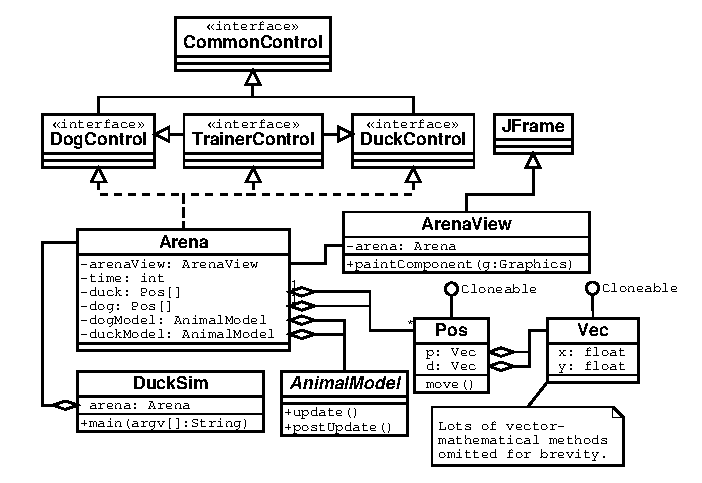
\includegraphics{figs/ducksim2.eps}}
  \caption{\label{fig-ducksim-uml}
    Simplified UML class diagram of \code{ducksim} package.
    Many attributes and methods are omitted for clarity.}
\end{figure}

\chapter{Neural networks for control}

\begin{quote}
  I have yet to see any problem, however complicated, which, when you
  looked at it the right way, did not become still more complicated.

  {\hspace{5cm}--- Poul Anderson}
\end{quote}

\section{Possible network architectures}

\label{net-archis}

With a simulation framework in place, the next step was to investigate
new algorithms for control. The aim was to use some form of neural
network controller, but this still leaves a bewildering choice due to
the huge variety of network architectures. An extensive survey of
neural network architectures and training algorithms suitable for
control systems is given in \cite{hunt92}.

One the best-known types of neural net is the multilayer feedforward
perceptron, most usually trained using backpropagation
\cite{rumelhart86}. A brief description of this method is given in
Section \ref{theory-ff-bp}. This was one of the first systems I
considered; however, both the architecture and the training algorithm
are, in their usual form, inadequate for this project. The standard
feedforward network cannot be used to model events with temporal
structure, since it has no internal memory and the outputs at any
point in time are entirely dependent on the inputs\footnote{Actually,
  time \emph{can} be modelled by feedforward nets, by representing it
  as an extra spatial dimension, but there are severe limitations with
  this approach (discussed in \cite{elman90}), making it unsuitable for
  this project.}. It is clear that, no matter what training algorithm
is used, the controller would always produce the same output in the
same situation: it would be impossible for it to develop the
higher-level strategies needed to control the flock.

Backpropagation as a training algorithm also has its drawbacks for
this task: with backpropagation, a network is trained by presenting it
with an input and comparing its outputs with the desired set of
outputs. However, in this situation the desired output is not as
clear as in, say, a pattern-recognition task. Rather, the correctness
is measurable only in terms of the \emph{effects} of the outputs on
the simulation over a period of time. Measuring the ``correctness'' of
a controller is relatively easy, by awarding scores for achieving
desirable tasks. Propagating this information back into the network is
harder, although complementary reinforcement backpropagation,
discussed in Section \ref{theory-crbp}, provides one solution.

Another way to extend backpropagation is discussed in \cite{widrow88}:
the rest of the simulation is also implemented as a neural network,
and is grafted onto the controller to be trained, the controller's
output nodes forming the inputs of the rest of the system.
Backpropagation is then applied as usual, but only the weights of the
controller are modified. Due to the complexity of reimplementing the
rest of the simulation as a neural net, and the relative paucity of
literature on this technique, I decided against attempting this.

\section{Simple recurrent networks (SRNs)}

The next stage was to investigate recurrent networks -- networks
containing connections which do not go strictly forwards from layer to
layer. This provides for much more capability in responding to inputs
which vary through time, but makes training more difficult and
time-consuming. One of the best-known techniques for training
recurrent nets, backpropagation through time, becomes very expensive
in time and memory when used for longer periods (\cite{rumelhart86},
p. 356).

An architecture which seems to offer many of the benefits of a
recurrent network without sacrificing ease of training is the Simple
Recurrent Network used by Jordan (\cite{jordan86}) and Elman
(\cite{elman90}). Although its most common application seems to be in
linguistic areas, where it can be trained to behave like a
finite-state automaton, it has also been used for controllers similar
to the one in this project (\cite{meeden96}).

The SRN architecture extends a standard 3-layer feedforward network by
adding a layer of \emph{context nodes}; a simple example is shown in
Figure \ref{fig-srn}. There are as many of these as there are hidden
nodes, and they act as a short-term memory for the hidden layer. Like
the input layer, the context layer has forward connections to the
hidden layer and is activated before the hidden layer during forward
propagation. However, the hidden layer also contains one-for-one
backlinks to the context layer (i.e. each hidden node is connected to
exactly one context node). These backlinks have a non-adjustable
weight of 1 and the context nodes use an identity activation function;
in other words, the hidden-layer activations are simply copied into
the context layer after they have been calculated.  The net effect is
that, on every forward-propagation pass, each hidden node is presented
with its own previous activation as one of its inputs. In spite of
this seemingly short-term memory, SRNs have proved capable of
developing fairly long behavioural patterns.

The SRN architecture adds another tunable parameter to those already
present in a standard feedforward network: the initial activations of
the context nodes. Usually these are reset to some neutral value, such
as $0.5$, at the start of every sequence of training patterns. The
longer the network is run for, the less significant these become, so I
didn't investigate the effects of changing their values.

\begin{figure}[htb]
  \centerline{\includegraphics{figs/srn.eps}}
  \caption{  \label{fig-srn} A simple recurrent network with two 
    input nodes, two hidden nodes, and two output nodes. The recurrent
    links to the context layer are shown as dotted arrows.}
\end{figure}

One of the attractive aspects of SRNs is that they can be trained by
simple backpropagation; during the backpropagation phase the context
nodes are just treated as another set of input nodes.  Meeden
(\cite{meeden96}) investigates two training methods, complementary
reinforcement backpropagation and a genetic algorithm, and I decided
to try the same methods for the dog controller. These methods are
described in more detail in Appendix \ref{theory-bg}, and in Sections
\ref{theory-crbp} and \ref{theory-ga-nn}.

\section{Coupling a neural network to the dog controller}

\label{impl-coupling}
A vital part of the project was the mechanism for actually associating
the network's input and output values with the motion of the dog: what
information to feed in, and how to interpret the outputs. An obvious
first step, both for input and output, was to translate the
simulation's Cartesian co-ordinates to polar ones relative to the
dog's current position. Intuitively it seems simpler to develop
control algorithms in terms of directions and distances than in terms
of $x$ and $y$ co-ordinates.

\paragraph{Input encoding} A good rule of thumb with neural networks
is never to use more neurons than necessary. Using too large a network
needlessly enlarges the space that learning algorithms have to search,
thus increasing training times. It can also cause overfitting to noisy
data or to specific training samples. I decided to experiment with a
few carefully selected and preprocessed values as inputs for the
network. I implemented functions to convert positions to a direction
and distance from the dog, both scaled to the range $[0,1]$.  The most
important data were the position of the nearest point on the wall
(vital to avoid colliding with it), the position of the flock centre,
and the radius of the flock. I also considered adding the position of
the closest duck, but decided to leave it out, at least initially.

\paragraph{Output encoding}

The network only needs to produce two values, controlling the dog's
speed and direction respectively. However there was still choice as to
the exact control method: should the speed (or angular velocity) be
applied directly, or should it be interpreted as an acceleration and
added to the current value? And to what ranges should the outputs be
scaled? Again, experimentation was needed. The results are discussed
in Section \ref{res-ga}.

\section{Implementing neural networks in Java}

The first step was to write a Java package to implement SRNs. In a
spirit of modularity, I kept this completely separate from the
\code{ducksim} package: the two packages only intersect in the neural
dog-controller class attached to \code{Arena}. I called my neural
network package \code{neurotic}; a UML class diagram of the final
version is shown in Figure \ref{fig-neurotic}.

There is a lot of choice as to the implementation of neural networks
in Java. Much of this is to do with the tradeoff between speed on the
one hand, and clarity and flexibility on the other. A fast solution
would be to store data such as weights and activations in arrays,
allowing them to be accessed quickly by training algorithms. However,
this implementation would be quite rigidly tied to a particular
network structure. Because I wanted the freedom to experiment with
different network architectures, and because I didn't anticipate using
networks of more than around a dozen neurons at most, I thought a
slower, more object-oriented approach would be most
suitable.\footnote{The (non-neural) duck controller turned out to be
  the bottleneck when training (see Section
  \ref{res-training-problems}) so this was probably the right choice.}

I made the obvious design choice of creating a \code{Neuron} class
representing a node in the network. At first I attempted storing the
link data within the nodes themselves, but this quickly became messy
since the data needed to be accessed from both ends of the link.
After some experimentation, I introduced a binary association class
\code{Link} representing a link between neurons.

Eventually I made \code{Neuron} a concrete subclass of an abstract
class \code{Axon}, which represents anything that can produce an
activation in a network. This encompasses input nodes, ``normal''
nodes like Neuron, and the context nodes used in SRNs.

The hard work of creating and running networks of these objects is
done by the \code{Net} class, representing an entire neural network.
It initializes a feedforward network or SRN based on parameters passed
to the constructor, and provides methods for setting the inputs,
running forward-propagation, and getting the ensuing outputs. The
most important methods and inner classes are:

\begin{itemize}

\item \code{Net}, the constructor, which creates a new 3-layer network
  (recurrent or feed-forward) with the number of nodes in each layer
  supplied as arguments.

\item \code{randomizeWeights(float mean, float range)} initializes
  every trainable weight in the network to a uniformly distributed
  random value with the given mean and range.

\item \code{setIn}, \code{getIn} and \code{getOut} are accessor
  methods for the input and output nodes.

\item \code{Activation} is a wrapper class around an activation
  function for the net, and \code{Sigmoid} is a private subclass
  giving the usual activation function. Since I didn't intend changing
  this, it is currently ``hard-wired'', but could easily be altered.

\item \code{LinkEnum} is a public inner class implementing the
  \code{Enumeration} interface. Instantiating it gives an enumeration
  over all the links in the network; it is useful both for
  \code{Net}'s internal methods and for other classes which might wish
  to read or modify weights.

\item \code{getAllWeights} and \code{setAllWeights} allow access to
  all the network's weights as an array, and \code{numWeights()}
  returns the number of weights in the network.

\item Various methods for training the network by backpropagation,
   described in Section \ref{impl-bp}.

\item Various methods for debugging.

\end{itemize}

\begin{figure}[htb]
  \centerline{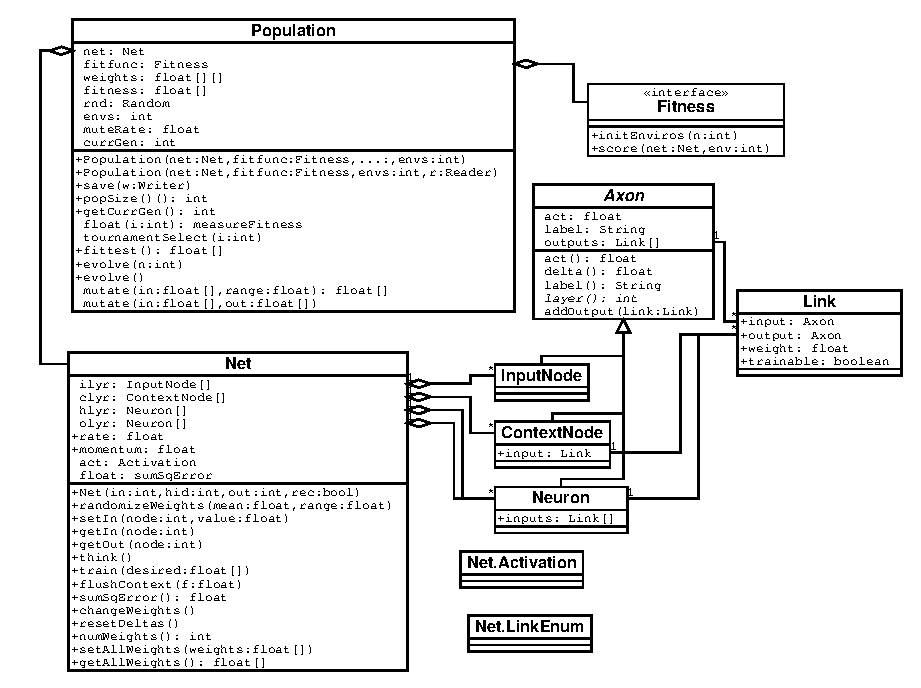
\includegraphics{figs/neurotic.eps}}
  \caption{\label{fig-neurotic} UML class diagram of \code{neurotic}
    package (some fields and methods are omitted for clarity).}
\end{figure}

\section{Training with backpropagation}

\subsection{Complementary reinforcement backpropagation}
\label{theory-crbp}

Complementary reinforcement backpropagation (CRBP), described in
\cite{ackley90}, is a method for getting around the problem discussed
in Section \ref{net-archis}: the fact that normal backpropagation can only
train a network on the basis of its actual outputs, against some other
set of desired outputs. CRBP provides a method for training a network
on the basis of a fitness function defined by the network's
interaction with some wider context.

The principle of CRBP is to extrapolate the network's actual output
vector to produce a ``virtual'' target vector against which to perform
the usual backpropagation algorithm. In slightly more detail, the
procedure is as follows:

\begin{enumerate}
  
\item Initialize the network randomly, as usual.
  
\item Run a forward propagation. Take the output vector from the
  network (the \emph{search vector}). Use it to construct a vector of
  equal length consisting of 0s and 1s, which \cite{ackley90} confusingly
  refers to as the \emph{output vector}. Each element $s_i$ of the
  search vector is interpreted as a probability; the corresponding
  element $o_i$ of the output vector is generated (pseudo-)randomly,
  taking the value 1 with probability $s_i$ and 0 otherwise.
  
\item Evaluate the performance of the `output vector', to produce a
  result indicating either that it is desirable and should be
  reinforced, or that it is undesirable and should be discouraged.
  
\item If the `output vector' is to be reinforced, it is simply used as
  the target vector for a backpropagation pass: the error vector
  $\mathbf{o} - \mathbf{s}$ is propagated through the network.
  
\item If the `output vector' is to be discouraged, it is slightly less
  obvious what to do: clearly the weights should be pushed away from
  the output vector, but in which direction? In the CRBP algorithm
  they are pushed in the exact opposite direction: the vector
  $\mathbf{(1-o)-s}$. Generally a lower learning rate is used here
  than for positive reinforcement, since the network is not
  necessarily being pushed towards a good set of values: it is merely
  being pushed away from a bad set.

\end{enumerate}

The procedure is repeated until the error has been
sufficiently minimized.

Although CRBP allows reinforcement methods to be used to train neural
networks, it is still geared towards immediate reinforcement: the
reinforcement value must be calculated after each forward-propagation
pass. There is no direct way to define a fitness function over a
longer sequence of behaviour. With a recurrent network, the network
itself can still develop longer-term strategies from short-term
reinforcement, but \cite{meeden96} gives discouraging results about
the difficulty of doing this. However, since most of the tasks I was
looking at lent themselves to immediate evaluation (for example, ``has
the size of the flock decreased?''), this was not too great a problem.

\subsection{Implementation of the backpropagation algorithm}
\label{impl-bp}

Since I intended to experiment with variations in the backpropagation
algorithm, I started with a fairly large, open interface to the
backpropagation methods. As it turned out, this interface remained in
place: the failure of backpropagation as an effective training method
(see Section \ref{results-bp}) meant that it was not worth improving
the interface.

Backpropagation works on a single network, so it made sense to
implement it using instance methods of the \code{Net}
class.\footnote{This is in contrast to the genetic algorithm discussed
  in the next section, which works on populations of networks and thus
  requires a somewhat different implementation strategy.} The main
public methods for controlling backpropagation are:

\begin{itemize}

\item \code{resetDeltas()} zeroes the accumulated weight changes built
  up over successive backpropagation passes.

\item \code{flushContext(float x)} sets the values of all the
  network's context nodes.

\item \code{train(float[] desired)} performs a forward-propagation
  pass followed by a backpropagation pass against the given target
  vector. It is assumed that the input values have already been set
  with the \code{setIn()} method. Weight changes are added to the
  internal accumulator variables, but not applied.

\item \code{changeInputWeights()} applies the weight changes
  accumulated during backpropagation.

\item \code{sumSqError()} returns the sum of squared errors computed
  on the last backpropagation pass.

\end{itemize}

The chief reason for separating out the calculation of weight changes
from their application is to make it easier to experiment with batch
and stochastic weight-update techniques (see page
\pageref{theory-bp-batch}).

\section{Genetic algorithms (GAs)}

A brief description of common GA techniques is given in Section
\ref{theory-ga}. The following sections describe the deviations from
``standard practice'' in my use of genetic algorithms, and the details
of their implementation in Java.

\subsection{Applying genetic algorithms to neural nets}

\label{theory-ga-nn}
I restricted the use of genetic algorithms in the project to evolving
the actual weights for the network, although there is scope for other
applications -- for example, determining the network architecture, or
adjusting parameters for other learning methods such as
backpropagation. However, I thought that using a genetic algorithm for
exactly the same task as CRBP would make for an interesting
comparison.

Following the approach of \cite{meeden96}, I ended up using a somewhat
unorthodox variant of genetic training, due to the unusual (for the
field of GAs) structure of the solutions I was attempting to evolve:

\paragraph{String encoding}
The first deviation from the norm is in the encoding of the strings
within a population. An individual in the population consists of a
string of floating-point numbers representing weights. Of course, it
would be possible to convert the weight values to bit-strings, but
this would bring no obvious benefits.

\paragraph{Crossover}
Crossover is not used at all. This may seem a little odd, but for
strings of weights it makes sense: the operation of a neural network
is highly distributed, with few or no easily identifiable ``modules''
in most cases. The ``parent'' networks may be using completely
different strategies to achieve the same goal. Even if they are not,
the same network architecture can produce the same behaviour using
radically different weights.\footnote{As a trivial example, consider a
  3-layer feedforward network with activations in the range $[-1,1]$.
  Provided the activation function is odd, simply negating all the
  weights will give a network with identical behaviour} so an
arbitrary substring of a ``good'' weight-string is unlikely to possess
any intrinsically good properties of its own.

In \cite{meeden96} it was found that, even if weights were grouped
into higher-level blocks to counteract this effect, crossover ``did
not improve and often hurt performance''. For this reason I decided
not to use crossover, at least not initially.

\paragraph{Mutation}
Mutation is used much more heavily than is usual. Partly this is
to compensate for the lack of crossover, and partly because
mutation need not be such a drastic process when the string elements
are continuous values rather than bits -- values can just be slightly
perturbed rather than flipped to the other of two possible states.

In practice, the mutation method used was a fairly brutal one, but one
which is successfully used in \cite{meeden96} and \cite{fogel98}:
\emph{every} weight in the string to be mutated is modified by a
random amount. \cite{yao99} also cites several successful applications
of similar techniques.  The range of modification is configurable by
the user, but in practice it was generally between 2 and 10 (that is,
$\pm 1$ to $\pm 5$).

\paragraph{Fitness function}
The fitness function was implemented in a slightly unusual way.
Instead of a wholly objective function which can assign an absolute
fitness to any set of weights, I used functions which evaluated a
network's fitness with respect to certain environments -- i.e., initial
states of the simulation. Given an initial state consisting of the
positions and velocities of the simulated animals, the fitness
function runs the simulation for a certain amount of time and assigns
scores based on its behaviour. For example, in most cases the
situation ``dog runs into wall'' would be awarded a negative score, in
order to encourage the propagation of networks which avoid this
behaviour.

One obvious danger with this method is that a network trained in a
specific environment will utilize the specific features of that
environment to perform successfully, and may well exhibit very poor
performance when placed in other environments. One way to counteract
this is to use a set of several training environments and take the
total or average score. The modification described below also helps.

\paragraph{Tournament selection}
The lack of an objective fitness function requires some modification
to the overall structure of the evolution algorithm. As discussed
above, it would be undesirable to train in a single environment; even
training in a fixed set of predefined environments would incur the
risk of overspecialization. For this reason, a new set of environments
was created at the start of every generation.

The technique used for creating new generations was \emph{tournament
  selection}. Pairs of individuals are randomly selected from the
population, and their fitnesses assessed in the current set of
environments. The loser (i.e. the individual with the lower fitness)
is replaced by a mutation of the winner. To advance evolution by one
generation, this procedure is repeated a number of times equal to the
population size. Since the environments are reinitialized at the start
of each generation, overspecialized individuals do not survive for
long.

\subsection{Implementing genetic algorithms in Java}

Genetic training proved remarkably simple to implement compared to the
intricacies of backpropagation. I added a class \code{Population} to
the \code{neurotic} package. This class is instantiated with a
\code{Net} and a fitness function, as well as a few training
parameters such as population and mutation rate. \code{Population}
stores arrays of floats representing weights (either initialized
randomly through the supplied network or loaded from a file) and plugs
them into the network when fitness needs to be assessed.

The fitness function supplied to the network is just an interface
consisting of two methods: \code{initEnviros(int n)} initializes the
requested number of environments (usually called once at the start of
each generation), and \code{score(Net net, int env)} returns the
fitness of the given net with respect to the given environment.

The rest of the class just implements the mutation and tournament
selection described in the previous section, and provides a few
accessor methods for things like the current fittest individual and
generation.

\chapter{Results of training}

\begin{quote}
  Among all the supervised learning algorithms, backpropagation is
  probably the most wi(l)dely used.
  
  {\hspace{5cm}--- Yann LeCun}
\end{quote}

\section{Backpropagation}
\label{results-bp}

Since backpropagation is a relatively involved algorithm with plenty
of scope for bugs in the implementation, I decided to start with some
simple tests and work up to the use of CRBP on recurrent networks.

\subsection{Non-recurrent networks}

The first step was to get backpropagation working reliably for
non-recurrent networks. The multilayer perceptron equivalent of
``hello world'' is the exclusive-or function\footnote{This is mainly
  because the XOR function can't be modelled by a single perceptron.}.
I successfully trained a non-recurrent network (2+2+1 neurons) to
model this function. Training times were highly dependent on the
learning rate and momentum parameters; with high values for both
(around 1.0 and 0.8 respectively) the network usually required a few
hundred passes through the training set to reach a sum of squared
errors below 0.001. The code for this example is given in Section
\ref{prog-test-bpxor}.

I compared the performance of my backpropagation routines with that of
PDP++, a publicly-available neural-net package written in C++. For the
XOR example, the behaviour of the two systems was completely identical
given the same starting conditions, so I was satisfied that
\code{neurotic} was fairly reliable on non-recurrent networks.

\subsection{Simple recurrent networks}

\label{res-bp-srn}

In a similar vein to the preliminary test for non-recurrent networks,
I decided to start by training an SRN on the function used in
\cite{elman90}: sequential exclusive-or. The idea is that a sequence
of inputs (1 or 0) is presented to the single input node of an SRN. The
input sequence is made up of a number of 3-element subsequences, with
the first two elements being random and the third being their
exclusive-or. The network has a single output, which is trained
against the next element in the sequence. Obviously the network can't
predict the first two elements of a subsequence, but Elman succeeded
in training it to predict the third element when the second was
presented.

I was unfortunately unable to do the same. In spite of extensive
experimentation with tunable parameters and repeated careful scrutiny
of the code for bugs, the network resolutely failed to
converge. Unfortunately \cite{elman90} is somewhat sketchy on the
details of the training process, and I was unable to find any more
detailed references on training SRNs with backpropagation.

\subsubsection*{Slight success with SRNs}

Eventually I scaled the training problem down to an even simpler one:
the network just needs to echo the previous input in the sequence.
Training from randomly initialized weights proved just as hopeless as
for the XOR problem. However, this problem was so simple that I had
little trouble working out a suitable set of weights by hand. This led
to some interesting results: I found that if I ran backpropagation
with an initial weight-set close enough to my known solution, it would
converge. This suggested to me that there was no fundamental problem
with the algorithm, but that some maladjustment of network or learning
parameters was preventing effective convergence. The program listing
is given in Section \ref{prog-test-bpparrot}; some sample output is
shown below.

\begin{verbatim}
Performance before training:

Input  ***..*...*....*.*..***..*.*.*.***..***...*....*..****.**.*..
Output ?*??.??..??...??.*.?*??.??.*.*.*?*.?*??..??...??.?*?*?.*???.

After 800 backprop passes

Input  **..*...**..*...*..*.*....**..**.*..**..*.**.***.*..*.*.***.
Output ***..*...**..*...*..*.*....**..**.*..**..*.**.***.*..*.*.***
\end{verbatim}

The program starts with a 1-2-1 network initialized with weights close
to the ones I calculated. It runs a test by sequentially feeding it 60
random inputs (either 1 or 0, shown as ``*'' and ``.'' respectively)
and showing the output (encoded as ``.'' for under 0.2, ``*'' for over
0.8, and ``?'' otherwise).

The network is then trained with backpropagation on another randomly
generated binary sequence. After 800 passes, there is a clear
improvement in the performance; Figure \ref{fig-bptrain} shows how the
11 weights in the network change with training.

\begin{figure}[htb]
  \centerline{\includegraphics{figs/pgraph2.eps}}
  \caption{ \label{fig-bptrain} Weights in the ``input-repeater''
    neural network of Section \ref{res-bp-srn}, plotted against number
    of backpropagation training passes.}
\end{figure}


I spite of this promising result, I had already spent a great deal of
time trying to get backpropagation working and could not afford to
pursue it any further.  I reluctantly abandoned the implementation of
CRBP and moved on to genetic algorithms.

\section{Genetic algorithm}
\label{res-ga}

There were two main areas of experimentation here: the actual
mechanism for coupling the neural network to the dog controller, and
the fitness function which pushes the network's weights towrds the
desired behaviour. In addition, there was scope for variation in the
parameters of the genetic algorithm -- for example, the population
size and mutation rate.

I created a new \code{AnimalControl} class called \code{DogBreeder},
which forms the link between the duck simulation and the
\code{neurotic} package. The constructor takes a \code{DogControl} and
a \code{TrainerControl}, for running and training the neural
controller respectively. On instantiation, \code{DogBreeder} creates a
network and a population of weights. It also creates a \code{DbPanel}
object, which provides a Swing interface allowing the user to control
the training of the networks. Facilities are provided to start and
stop evolution (which takes place as a background thread), and to
alter parameters such as the population size and the number of hidden
nodes. The actual \code{update()} function which controls the dog's
movement is delegated to a servant class implementing
\code{DogBreeder.ControlInterface} (which is essentially just a
wrapper for \code{update()}), since I was making a lot of
modifications to this part.

The Swing GUI for the \code{DogBreeder} class is shown in Figure
\ref{fig-ga-ui}.

\begin{figure}[htb]
\centerline{\includegraphics{figs/ga-ui.pdf}}
\caption{\label{fig-ga-ui}The user interface for the \code{DogBreeder}
class.}
\end{figure}

\subsection{Avoiding walls}

I thought a good preliminary test for the genetic training method
would be wall avoidance: the fitness function just imposes a heavy
penalty (negative score) for running out of the arena. With only this
criterion the most likely result is a dog which doesn't move at all,
so the fitness function also adds a positive score proportional to the
distance moved over the training period.

I experimented with both direct mappings of the outputs to speed and
direction, and with using them as increments to be added on. I also
experimented with different scaling factors for the outputs. The goal
proved easy to achieve, whatever the exact system used.

The best performance seemed to result from mapping one output directly
to the dog's speed, and using the other as an increment to the
direction. This was the system I used for most of the later
experiments.

\code{AvoidWallsFitness}, the fitness function I developed for this
task, is listed in Section \ref{code-fit-avoid}. In operation, the
controllers it produces tend to move around the arena in circles,
although I did also find variants which had a more radial pattern of
movement.

\subsection{Training problems}

\label{res-training-problems} The two main problems I had with genetic
training were closely interrelated. The first was the speed of the
simulation. For real-time running of the simulation, my implementation
had proved more than fast enough. However, the genetic training was
much more computationally intensive; it takes hundreds or thousands of
simulation steps to evaluate the fitness of a single individual in a
population. This was not a great problem for the wall-avoidance task,
since there was no need to involve the ducks in the simulation.
However, as soon as I started tackling problems involving ducks,
training times shot up -- the duck controller consumed the bulk of the
processor time simply because there were so many ducks. Depending on
the exact parameters, a generation took from thirty seconds to two or
more minutes.

The second problem was with specifying fitness functions. I already
mentioned the success of the ``do nothing'' tactic in avoiding walls;
similarly degenerate solutions tended to crop up to more complex
problems. The solution is to empirically tweak the relative scores
assigned by the fitness function to specify the desired behaviour more
exactly. The problem with this is that the speed of evolution makes each
refinement cycle slow, so it can take a great deal of time to arrive
at an effective fitness function.

\subsection{Herding}

In spite of these setbacks, I eventually succeeded in producing a
neural controller which can herd ducks, albeit imperfectly.  The
fitness function, \code{HerdDucksFitness}, is listed in Section
\ref{code-fit-herd}. The main points of interest are:

\begin{itemize}

\item When initializing environments, the simulation is run for about
  a hundred steps with no dog motion. This compensates for the ducks'
  natural tendency to flock even without a herder, by allowing them to
  settle down.

\item As before, the dog is punished for hitting walls, and rewarding
  for moving.

\item The actual herding criterion is calculated by summing the ducks'
  distances from the goal (here, the arena's centre). At the end of
  the training period the sum is recalculated. The decrease in total
  distance is multiplied by a suitable factor and added to the score.
  
\item The inputs to the network were: the angle and distance to the
  nearest wall point; the angle and distance to the flock centre; and
  the maximum radius of the flock (i.e. the greatest distance of a
  duck from the flock centre). Thus the herding strategy was developed
  without knowledge of any individual duck positions.

\end{itemize}

In order to show the controller's behaviour over time, I instrumented
the \code{ArenaView} class to draw a trail behind the dog. Figure
\ref{fig-herd} shows the result of 88 generations of
training\footnote{The other parameters were: population size 48,
  hidden nodes 5, initial weight mean 0, initial weight range 4,
  mutation rate 4, training environments 40, and simulation steps per
  environment 80.} with \code{HerdDucksFitness}. The results are not
perfect, but are definitely promising. It is interesting that the
``spiralling'' strategy evolved is similar to that developed by
Vaughan in \cite{vaughan98}.

\pagebreak[4]
\begin{figure}[p]
\begin{tabular}{cc}
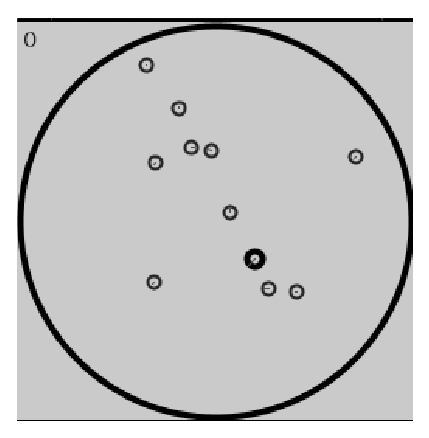
\includegraphics{screenshots/0.eps} & 
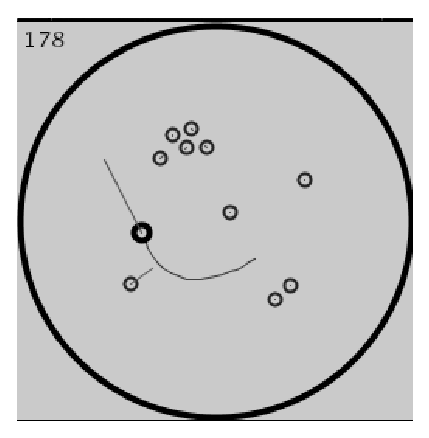
\includegraphics{screenshots/178.eps} \\
\parbox{65mm}{The dog starts in the middle\ldots} &
\parbox{65mm}{\ldots and rapidly begins to spiral outwards.} \\
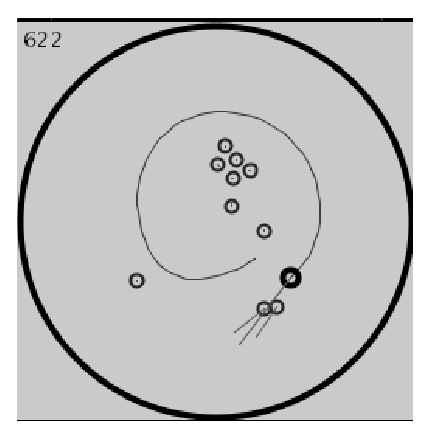
\includegraphics{screenshots/622.eps} & 
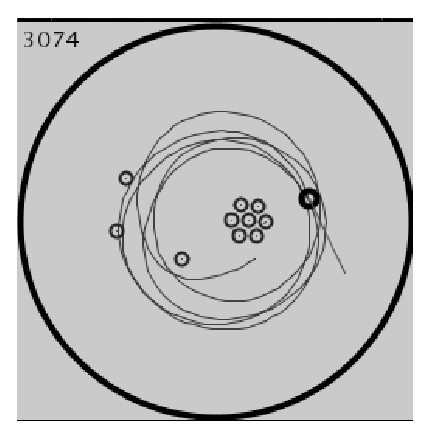
\includegraphics{screenshots/3074.eps} \\
\parbox{65mm}{The dog widens the spiral in an attempt to enclose all
  the ducks.} &
\parbox{65mm}{The radius of the spiral changes constantly in response to
  the flock size, but three ducks are still left out.} \\
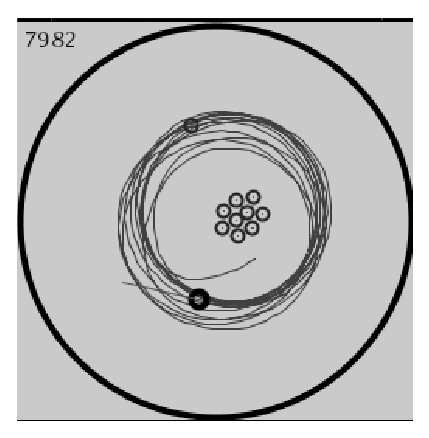
\includegraphics{screenshots/7982.eps} & \\
\parbox{65mm}{Eventually, all but one of the ducks have been
  successfully herded.} & \\
\end{tabular}
\caption{\label{fig-herd}The genetically developed herding algorithm in action}
\thispagestyle{empty}
\end{figure}

\chapter{Conclusions}

\begin{quote}
  A conclusion is just the place where you got tired of thinking.

  {\hspace{5cm} --- Martin H. Fischer}
\end{quote}

\section{Results of the project}

\paragraph{A duck simulation framework} The \code{ducksim} package
provides a pleasantly modular, object-oriented framework for
implementing and developing duck and herder control algorithms.

\paragraph{Reimplementation of previous work} The core parts of the
previous duck simulator were tidied up and re-implemented within the
new framework.

\paragraph{The \code{neurotic} package} A general-purpose package was
written for creating and using neural networks (both feedforward and
simple recurrent), with facilities for training them using
backpropagation and genetic methods.

\paragraph{A dog controller} Genetic training was applied to
develop a controller capable of herding ducks into the centre of the
arena.

\section{What I learned from the project}

\paragraph{Animal behaviour} The background to the project taught me
some basics of animal flight and flocking behaviour, how it may be
encoded algorithmically, and how it may be utilised for herding.

\paragraph{Neural networks} Prior to starting this project I knew very
little about neural networks. The research in the initial stages gave
me an overview of the field. Writing \code{neurotic} gave me a good
understanding for feed-forward and simple recurrent networks, and of
backpropagation. I also learned the principles of genetic algorithms,
and about their application to neural networks.

\paragraph{Java, OOP, and OOD} This is the largest project I
have ever undertaken in Java and my first experience with Swing. The
project gave me a chance to apply the object-oriented design
techniques from the II.4 Object-Oriented Programming course.  Both the
duck simulation and the implementation of neural networks involved
some careful object-oriented design (and sometimes redesign, after
finding limitations in the initial implementation).

\paragraph{Research skills} This was my first real experience of 
independent research. I have had to gather information from a wide
variety of sources -- books, journals, conference proceedings,
technical reports, web pages, FTP sites and the assembled wisdom of
the \texttt{comp.ai.neural-nets} newsgroup.

\section{Areas for further investigation}

Due to the limited time available for the project there were several
areas I was unable to investigate:

\paragraph{Motivational units} The previous dog algorithm, in contrast
to the neural controller, worked in a large number of distinct stages
or steps. Effectively the highest level was a finite state automaton,
switching states when certain conditions in the simulation were
met. Multi-stage behaviour such as ``make the flock size sufficiently
small, then move the flock towards the goal'' is difficult for a
neural network to model directly, but \cite{cecconi92} suggests a
solution in the form of a \emph{motivational unit} -- an extra input
node which, rather than being influenced directly by the environment,
is set by a user or a higher-level control algorithm. The network can
learn different modes of behaviour depending on the state of the
motivational unit.

\paragraph{Evolution of flocking behaviour}

This wasn't really a goal of the project, but could form an
interesting extension. Flocking behaviour in real animals has evolved
because it improves the animals' chances of survival, particularly
when faced with predators. There have been successful attempts, such
as \cite{werner-dyer92}, to recreate this evolution in
neurally-controlled simulated animals. It would be interesting to
evolve a neural controller for ducks in the presence of a simulated
predator, and compare its behaviour with that of the duck algorithm
constructed in \cite{vaughan98}.

\paragraph{Faster training} When I started using the genetic training
algorithm it soon became clear that the slowness of training was the
main obstacle to developing good genetic controllers. The main
bottleneck seemed to be in the duck updating: I obtained a significant
improvement by hand-optimizing the duck controller. Apart from using
faster hardware or rewriting the whole thing in a fully compiled
language, there are several feasible ways of improving performance:
profiling and more optimizing; natively compiling speed-critical parts
and interfacing them to the simulator with JNI; and running
parallelized versions of backpropagation and genetic training on
several machines at once (both these techniques lend themselves well
to efficient parallelization).

\paragraph{The user interface} The user interface was not intended to
be a major part of the project, so I did not spend much time on
it. There are many possible improvements, particularly regarding the
genetic training algorithm. A user could be employed to supplement the
fitness function by selecting and evaluating networks from the
population. There is also scope for presenting the user with much more
detailed information about the state of the population and of the
individuals; an animated display of a working neural net might prove
illuminating or, at any rate, pretty.

One neat enhancement would be using the Java reflection API to enable
dynamic loading of dog and duck controllers; different controllers
could be used without the need for recompilation. This would also
speed up the development of algorithms.

\appendix

\chapter{Background information}
\label{theory-bg}
\section{Feedforward networks and backpropagation}
\label{theory-ff-bp}

\subsection{Structure of feedforward networks}

An artificial neural network is made up of a set of nodes $U = \{u_1,
\ldots, u_n\}$. Any two nodes $u_i$ and $u_j$ may be connected by a
directed arc, which has an associated real-valued weight $w_{ij} : i,j
\in \{1, \ldots, n\}$. The backpropagation algorithm works with a
particular type of \emph{feedforward} network: in this network
architecture, nodes are organised into layers, and a link from a
node may only connect to a node in a layer strictly above it in the
network. Thus the network is acyclic. An example of a three-layer
feedforward network is shown in figure \ref{fig-ffn}.

\begin{figure}[htb]
  \label{fig-ffn}
  \centerline{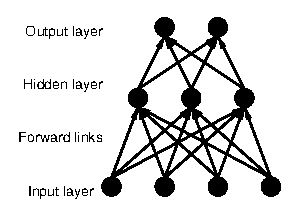
\includegraphics{figs/ffn.eps}}
  \caption{An example of a feedforward network}
\end{figure}

Associated with each node is a number, its \emph{activation}. For
backpropagation networks this is usually a real in the range $[-1,1]$
or $[0,1]$. (My implementation uses $[0,1]$.) The bottom layer in the
network (the one into which no arcs are directed) is termed the
\emph{input layer}; the activations of its nodes are set externally
and form the input of the network. Predictably, the topmost layer is
called the \emph{output layer} and the activations of its nodes will
form the network's output.

For a node $u_i$ not in the input layer, the activation is computed as a
function of the activations of the nodes $u_j$ for which links from
$u_j$ to $u_i$ exist. A weighted sum is taken of the activations, and
a predefined \emph{activation function} $f$ is applied to this sum to give
$u_i$'s activation. The activation $a(u_i)$ is given by

\[ a(u_i) = f(\sum a(w_{ji})u_j) \]

There is one other factor in the activation of a node: its
\emph{bias}. This is simply a constant which is added to the weighted
input sum before the activation function is applied. The easiest and
most common way of implementing bias, and of allowing it to be
modified by training algorithms, is to add an input node with a
constant non-zero activation (usually 1) and make connections from it
to all the hidden and output nodes in the network. The weights of
these connections can then be adjusted by training algorithms just
like any other weights in the network.

Since there is no restriction on the range of the weights and the
activation must be in the range $[0,1]$, the activation function must
map $[-\infty, \infty]$ to $[0,1]$. Additionally, for backpropagation
to work, it must be monotonic and continuous. The most commonly used
function (and the one I use) is the logistic function $f(x) =
\frac{1}{1 + e^{-x}}$.

The process of computing a function using a neural network simply
consists of setting the input activations to the input values, then
successively computing the activations for nodes in subsequent
layers. The activations for the nodes in the final layer form the
output.

\subsection{The backpropagation algorithm}

Backpropagation is an algorithm for adjusting the weights of a
feedforward network in order to make it model a particular function.
It minimizes error by gradient descent: starting from a random point
in weight-space, it ascertains the gradient of the error function and
adjusts the weights in that direction, working towards a minimum.
Unfortunately the minimum is not guaranteed to be global, but it is
nevertheless a powerful algorithm.

In outline, backpropagation works like this:

\begin{enumerate}

\item A training set is assembled, consisting of sample inputs for
  network, with a desired output for each input. The weights of the
  network are initialised to small random values.

\item The network is presented with an input from the training set,
  and a forward-propagation is run to produce output values.

\item The difference is calculated between the actual output values
  and the desired outputs from the training set. These error values are
  propagated backwards through the network, allowing changes in the
  weights of the connections to be calculated.

\item The weights of the connections are altered.

\item Steps 2-4 are repeated until the network models the desired
  function with sufficient accuracy.

\end{enumerate}

In slightly more detail, the backprpagation pass works as follows:

\begin{enumerate}
  
\item Take the derivative of the activation function. If the usual
  logistic function is used, then the identity $f'(x) \equiv
  f(x)(1-f(x))$ can be employed to speed up calculation by using the
  previously computed activations.
  
\item Associate with each node $u_i$ a real number $\delta_i$.
  
\item For each node $u_i$ in the output layer, calculate $\delta_i$ by
  $\delta_i = (C_i - a_i)f'(S_i)$, where $C_i$ is the correct target
  activation for that node, and $S_i$ is the weighted sum used as
  input to the activation function (so actually $\delta_i = (C_i -
  a_i)a_i(1-a_i)$).
  
\item Now move backwards through the network's hidden layers. For each
  node compute $\delta_i = (\sum_j w_{ij}\delta_j)f'(S_i)$, where the
  $j$ range over all the nodes to which forward connections run from
  $i$. Since each $\delta_i$ value only depends on those of the nodes
  in front of it in the network, they can all be computed consistently
  in a single backward pass.

\item Finally, update each weight $w_ij$ with the new value $w_ij +
  \rho \delta_j a_i$. $\rho$ is the learning rate, usually in the
  range 0--1 (see below).

\end{enumerate}

There are numerous variations of the algorithm, and several tunable
parameters which affect its performance. Some of the main variations,
most of which were incorporated into my simulation, are:

\begin{itemize}

\item The actual layout of the network. The number of input and output
  nodes is largely determined by the function which the network is
  being trained to compute, although in this project there is
  considerable choice as to how the inputs and outputs should be
  encoded (see Section \ref{impl-coupling}). The number of hidden
  nodes, however, is an important tunable parameter: too few will
  result in the network being unable to model the desired function,
  and too many will make learning slow and unreliable.
  
  The number of layers is another tunable parameter, but I have kept
  it at three (four including the context nodes) for this project.
  
\item The distribution of the initial random weights, which can have a
  significant effect on the solution which the network converges to.
  
\item A \emph{momentum} parameter can be added to the direction of
  gradient descent, allowing the algorithm to pick up speed if it
  makes many consecutive changes in the same direction. This can speed
  up learning significantly, but can also lead to minima being missed.
  
\item The \emph{learning rate} is a fixed factor governing how much
  the weights are adjusted at each step. Lower values give slower but
  more reliable convergence.
  
\item Instead of updating the weights at each iteration (this is known
  as \emph{stochastic} update), the $\delta_i$ values can be
  accumulated over many iterations, or over the whole training set,
  and only applied at the end (\emph{batch} update).\label{theory-bp-batch}

\end{itemize}

\section{Genetic training}
\label{theory-ga}

Genetic algorithms are conceptually simple, but are widely applicable
and can prove highly effective. The method is modelled on the
principle of natural selection. It can be employed on virtually any
problem where (1) the parameters of a possible solution can be encoded
as a relatively compact sequence of numbers or symbols and (2) there
exists a \emph{fitness function} or \emph{objective function} which
can assign a numerical value reflecting how ``good'' a candidate
solution is.\footnote{The satisfaction of these two criteria does not,
  of course, guarantee that a particular genetic algorithm will work!}

Genetic algorithms come in numerous variations, but given a suitable
problem the general procedure is as follows\footnote{This summary is
  based on the descriptions given in \cite{wasserman93} and 
  \cite{winston92}.}:

\begin{enumerate}

\item Devise a way of encoding the parameters of a solution into a
  fixed-length string or numbers or symbols. Very often, binary digits
  are used, but this is by no means mandatory. The choice of encoding
  method can have a huge impact on the performance of the algorithm.

\item Initialize a set of randomly generated strings, called the
  \emph{population} for obvious reasons.

\item Repeatedly apply the following three techniques:

  \begin{enumerate}
    
  \item \emph{Reproduction}: Assess the fitness of each individual in
    the population, and produce a ``weighted copy'' of the current
    population. That is, initialize a new population of the same size
    by, for each string, copying a string selected at random from the
    old population. The selection is linearly weighted by fitness, so
    that fitter strings have a higher chance of being selected.

  \item \emph{Crossover}: select pairs of strings from the
    population. For each pair, randomly select a point within the
    length of a string. Break both strings at this point, and exchange
    their final segments. For example, \texttt{001122} and
    \texttt{222333} might be split and recombined halfway to give
    \texttt{001333} and \texttt{222122}.
    
  \item \emph{Mutation}: perturb one or more strings. A string is
    selected at random, an element selected at random within that
    string, and a random modification applied to that element.
    Traditionally this method is used very sparingly; mutation rates
    of the order of one in a thousand are common.
 
  \end{enumerate}

\end{enumerate}

The genetic algorithm used in this project deviates somewhat from this
standard outline; the differences are described in Section
\ref{theory-ga-nn}.


{
\pagebreak
\setlength{\oddsidemargin}{0.0cm}
\setlength{\marginparwidth}{0cm}
\setlength{\textwidth}{18cm}
\setlength{\linewidth}{18cm}
\setlength{\hoffset}{-1.04cm}

\chapter{Source code}

\section{\code{ducksim} package}
%Due to space limitations, the \code{ArenaView} class and
%\code{DbPanel}, \code{DogBreeder}'s GUI class, are omitted.
\rule{\linewidth}{0.3pt}
\begin{multicols}{2}
  \subsection{DuckSim}
  \lgrindfile{pretty/ducksim/DuckSim}
  \subsection{Arena}
  \lgrindfile{pretty/ducksim/Arena}
  \subsection{ArenaView}
  \lgrindfile{pretty/ducksim/ArenaView}
  \subsection{ChengDucks}
  \lgrindfile{pretty/ducksim/ChengDucks}
  \subsection{DogBreeder}
% \lgrindfile{DogBreeder2}
  \lgrindfile{pretty/ducksim/DogBreeder}
  \subsection{DogControlIface}
  \lgrindfile{pretty/ducksim/DogControlIface}
  \subsection{AvoidWallsFitness}
  \label{code-fit-avoid}
  \lgrindfile{pretty/ducksim/AvoidWallsFitness}
  \subsection{HerdDucksFitness}
  \label{code-fit-herd}
  \lgrindfile{pretty/ducksim/HerdDucksFitness}
  \subsection{Vec}
  \lgrindfile{pretty/ducksim/Vec}
  \subsection{Pos}
  \lgrindfile{pretty/ducksim/Pos}
\end{multicols}
\pagebreak[1]
\section{\code{neurotic} package}
\rule{\linewidth}{0.3pt}
\begin{multicols}{2}
  \subsection{Axon}
  \lgrindfile{pretty/neurotic/Axon}
  \subsection{Link}
  \lgrindfile{pretty/neurotic/Link}
  \subsection{Net}
  \lgrindfile{pretty/neurotic/Net}
  \subsection{Fitness}
  \lgrindfile{pretty/neurotic/Fitness}
  \subsection{Population}
  \lgrindfile{pretty/neurotic/Population}
\end{multicols}
\section{\code{testsuite} package}
\rule{\linewidth}{0.3pt}
\begin{multicols}{2}
  \subsection{XorBP}
  \label{prog-test-bpxor}
  \lgrindfile{pretty/testsuite/XorBP}
  \subsection{BPparrot}
  \label{prog-test-bpparrot}
  \lgrindfile{pretty/testsuite/BPparrot}
\end{multicols}
\pagebreak}

\bibliographystyle{alpha} \nocite{*} \bibliography{biblio}

\end{document}

